This chapter describes the method proposed in this work for evaluating assistive devices using virtual reality. The method is organized into 5 phases, further decomposed into 10 steps, as illustrated in Figure \ref{fig:diag_metodologia}.


%\begin{figure}[!htb]
    \centering
    \tikzstyle{every node}=[font=\large]
    
    \tikzstyle{task} = [rectangle, rounded corners, minimum width=4cm, minimum height=1.5cm,text centered, draw=black, fill=white!30, text width=3.5cm, font=\large]
    \tikzstyle{phase} = [rectangle, minimum width=4cm, minimum height=1.5cm,text centered, draw=black, fill=white!30, text width=5.0cm, font=\Large]
    \tikzstyle{--gray} = [ccmLGray, dashed, dash pattern=on 1cm off 1cm , rounded corners, line width = 2mm]
    \tikzstyle{--red} = [ccmRed, rounded corners, line width = 2mm]
    \tikzstyle{--blue} = [ccmDBlue, rounded corners, line width = 2mm]
    
    \tikzstyle{arrow_blue} = [ccmDBlue, rounded corners, line width = 2mm, ->]
    \tikzstyle{d--blue} = [ccmDBlue, dashed, dash pattern=on 1.0cm off 0.65cm, rounded corners, line width = 2mm]
    \tikzstyle{arrow_--_blue} = [ccmDBlue, dashed, dash pattern=on 1.0cm off 0.65cm, rounded corners, line width = 2mm, ->]
    \tikzstyle{arrow_red} = [ccmRed, rounded corners, line width = 2mm, ->]
    
    
    \resizebox{\linewidth}{!}{
    \begin{tikzpicture}[node distance=1cm]
        
        \node (interview) [phase] {Phase 1 – Context definition:};
        \node (interview_hospital) [task, below of = interview, yshift = -2cm] {1.1 Interview with environment specialists;};
        \node (interview_bvi) [task, below of = interview_hospital, yshift = -3.5cm] {1.2 Interview with BVI consultants.};
        
        \node (a1) [right of = interview, above of = interview, xshift = 2.0cm] {};
        \node (a2) [below of = a1, yshift = -11cm] {};
        \draw [--gray] (a1) to (a2);
        
        \node (scope) [phase] [phase, right of = interview, xshift = 5cm] {Phase 2 – Specification:};
        \node (virtual_environment) [task, below of = scope, yshift = -2cm] {2.1 Virtual environment specification;};
        \node (human_factors) [task, below of = virtual_environment, yshift = -2cm] {2.2 Assessment specification;};
        \node (guidance_methods) [task, below of = human_factors, yshift = -2cm] {2.3 Guidance specification.};
        
        \node (b1) [right of = scope, above of = scope, xshift = 2.0cm] {};
        \node (b2) [below of = b1, yshift = -11cm] {};
        \draw [--gray] (b1) to (b2);
        
        \node (development) [phase] [phase, right of = scope, xshift = 5cm] {Phase 3 – Development:};
        \node (ve_creation) [task, below of = development, yshift = -2cm] {3.1 Implementation of virtual environment;};
        \node (tools_definition) [task, below of = ve_creation, yshift = -2cm] {3.2 Proposal of assessment techniques and tools;};
        \node (guidance_development) [task, below of = tools_definition, yshift = -2cm] {3.3 Development of guidance devices.};
        
        \node (c1) [right of = development, above of = development, xshift = 2.0cm] {};
        \node (c2) [below of = c1, yshift = -11cm] {};
        \draw [--gray] (c1) to (c2);
        
        \node (tryouts) [phase] [phase, right of = development, xshift = 5cm] {Phase 4 – Preliminary evaluation:};
        \node (tryouts_task) [task, below of = tryouts, yshift = -5.0cm] {4.1 Try-outs.};
        
        \node (d1) [right of = tryouts, above of = tryouts, xshift = 2.0cm] {};
        \node (d2) [below of = d1, yshift = -11cm] {};
        \draw [--gray] (d1) to (d2);
        
        \node (experiment) [phase] [phase, right of = tryouts, xshift = 5cm] {Phase 5 – Systematic evaluation:};
        \node (experiment_task) [task, below of = experiment, yshift = -5.0cm] {5.1 Controlled experiments.};
    
        \draw[arrow_blue] (interview_hospital.east) to (virtual_environment.west);
        \draw[arrow_blue] (interview_bvi.east) to ++(1.0,0) to ++(0,4.5) to (virtual_environment.west);
        \draw[arrow_blue] (interview_bvi.east) to ++(1.0,0) to ++(0,1.5) to (human_factors.west);
        \draw[arrow_blue] (interview_bvi.east) to ++(1.0,0) to ++(0,-1.5) to (guidance_methods.west);  
        
        \draw[arrow_blue] (virtual_environment.east) to (ve_creation.west);
        \draw[arrow_blue] (human_factors.east) to (tools_definition.west);
        \draw[arrow_blue] (guidance_methods.east) to (guidance_development.west);
        
        \draw[arrow_blue] (ve_creation.east) to ++(1.0,0) to ++(0,-3.0) to (tryouts_task.west);
        \draw[arrow_blue] (tools_definition.east) to ++(1.0,0) to  (tryouts_task.west);
        \draw[arrow_blue] (guidance_development.east) to ++(1.0,0) to ++(0,3.0) to (tryouts_task.west);
        
        \draw[arrow_blue] (tryouts_task.east) to (experiment_task.west);
        \draw[--red] (tryouts_task.north) to (tryouts.south);
        \draw[--red] [opacity=0.2] (tryouts.south) to (tryouts.center) to (tryouts.west);
        \draw[arrow_red] (tryouts.west) to (development.east);

        \draw[d--blue] (experiment_task.north) to (experiment.south);
        \draw[d--blue] [opacity=0.2] (experiment.south) to (experiment.center) to (experiment.north);
        \draw[arrow_--_blue] (experiment.north) to ++(0,1.0) to ++(-18.0,0.0) to (scope.north);
        
    \end{tikzpicture}
    }
    \caption{Method's diagram}
    \label{fig:diag_metodologia}
\end{figure}

\begin{figure}[H]
    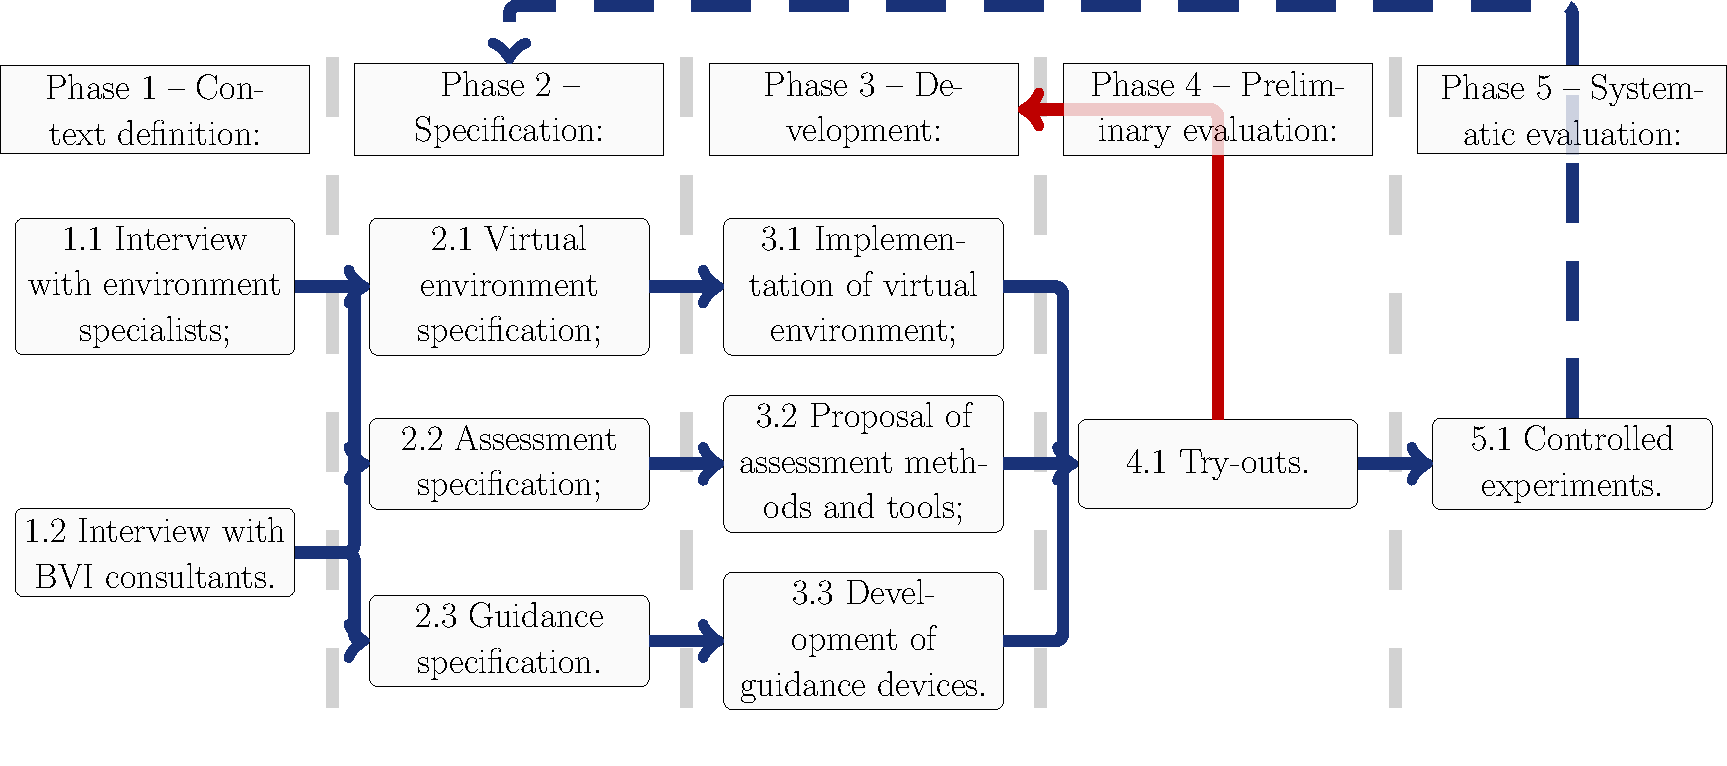
\includegraphics[width = \linewidth]{Metodologia/metodologia.pdf}
    \caption{Method's diagram}
    \label{fig:diag_metodologia}
\end{figure}

The first phase is the context definition. It consists of defining the main features of the environment in which the assistive device will be used, based on interviews from specialists. It also includes a step for understanding the limitations of the current assistive devices and defining the main features of assistive devices to be designed. This last step is based on interviews with BVI users.

The second phase is devoted to specification and is composed of three steps. It includes the specification of a virtual environment that represents the real environment where the device will be used. In parallel, the relevant human factors for the device evaluation are defined. Finally, the assistive devices are also specified.

The third phase is dedicated to developing the virtual environment, the evaluation tools and techniques, and the first proof of concept of the assistive devices, which should be integrated into the virtual environment for testing. 

The fourth phase provides a preliminary assessment of the devices through its unstructured experimentation by BVI consults. This preliminary assessment provides feedback for improving the device concept. The cycle of “try-out and improve device concept” can be repeated until the device concept is considered mature to be tested through a systematic set of controlled experiments.

The fifth phase consists of executing a campaign of controlled experiments, following the best practices of the DoE (Design of Experiments) discipline, and analysing the results. Concluded this phase, the results should provide information for the design team to decide between proceeding to the detailed design of the assistive devices or performing a new evaluation cycle.

In the last case, the experiment should provide feedback on improving the devices' specification, refine the assessment techniques, expand the virtual environment to include new tasks and/or situations, or even abandon a device concept. Each evaluation cycle should increase the maturity of the assistive devices under development.

In order to illustrate it, the proposed method is applied to the evaluation of assistive devices concepts that should be able to guide BVI users in a hospital or a medical clinic during the covid-19 pandemic.

\section{Phase 1 – Context definition}
\label{sec:interviews_phase}
    As previously stated, the context in which the assistive devices are evaluated is the BVI navigation through a hospital or medical clinic in a covid-19 pandemic situation. 

    \subsection*{\textit{Step 1.1 Interview with environment specialists}}
    
        In order to gather information about this context, the first step of Phase 1 consists of interviewing specialists from hospitals to understand the usual hospital procedures and the standard features of this environment.
        
        For this work, employees from two hospitals of São José dos Campos were interviewed (Vivalle Hospital and the Municipal Hospital). They were questioned about the layout of rooms and spaces and the processes that a new patient follows through the hospital, from the check-in until he/she gets in the doctor's office. 

        According to the interviews, the procedures adopted by patients in both hospitals are similar and are usually composed of the following steps:

        \begin{enumerate}
            \item Enter the hospital;
            \item Use the sanitizer to clean their hands;
            \item Take a queue number and wait for the call of the receptionist;
            \item Go to the receptionist and check in;
            \item Sit in the waiting area and wait until the patient's name is called;
            \item Leave the waiting area toward the doctor's office.            
        \end{enumerate}


    \subsection*{\textit{Step 1.2 Interview with BVI consultants}}
    
        One of the motivations of this work is that BVI users are not completely satisfied with the current guidance products. We hypothesize that BVI users are not usually consulted from the early stages of the products' development.

        In this work, two BVI acted as consultants for the proposal of guiding devices and the design of a virtual environment that would be familiar to their reality. They had different visual impairments. One of them became blind at the age of 13 years old, while the other was diagnosed with Usher's disease. 

        The interviews with BVI consultants were critical to understanding how they perceive a medical clinic as they walk in and how they interact with the environment. Among the inputs provided by BVI interviews' are the importance of including in the virtual environment background noise typical of a reception, such as a keyboard typing and a telephone ringing, as well as a few physical expected objects to interact with (chairs and desk).
    

\section{Phase 2 - Specification}
\label{sec:idealization_phase}
    In Phase 2, the information collected through the interviews of Phase 1 is used to make critical decisions about the virtual environment where the evaluation of the assistive devices will be carried out. It is also used to define which human factors should be assessed. Finally, it contributes to define the guidance devices that should be implemented in the assistive devices.
    

    \subsection*{\textit{Step 2.1 Virtual environment specification}}
        Based on the data collected during the interviews, the scenario was defined as the hospital or medical clinic reception. The BVI patient should be able to navigate through the reception hall and reach a reception desk. After he/she is registered, the BVI patient should wait until he/she is called and then goes to his/her doctor's office.

        At this step, a preliminary layout of the virtual environment was sketched, combining the elements that were common to the reception of the two hospitals, such as a waiting area with chairs (some of which should remain empty due to covid distancing), a reception desk, an alcohol totem, among others.

        One limitation that had to be taken into account in the specification of the virtual environment is the corresponding physical area (real empty room) that should be available so that the BVI could walk through the real world. while he/she navigates in the virtual world. Typical dimensions of a reception are around 15x20m. Due to the limited space available at the laboratory, the reception was scaled down to fit into the available physical space, with an area of 7x10m but maintaining the same elements (reception desk, waiting area, sanitizer, among others)
    

    \subsection*{\textit{Step 2.2 Assessment specification}}
        Based on the review of the literature and the BVI interviews, the assessment techniques should include the following dimensions, which were commonly evaluated in previous works: 

        \begin{enumerate} [label = \Alph*)]
            \item Performance evaluation;
            \item Mental workload evaluation.
        \end{enumerate}
            
        Additionally, a third dimension was also included, based on lessons learned from the Aeronautics area:   

        \begin{enumerate} [label = \Alph*)]
            \setcounter{enumi}{2}
            \item Situation awareness evaluation.
        \end{enumerate}
            
        This dimension was included to verify if the BVI user can build a mental map of the environment based on the inputs provided by the devices.

        Finally, a fourth dimension is included for evaluating the user preferences when comparing the assistive devices.

        \begin{enumerate} [label = \Alph*)]
            \setcounter{enumi}{3}
            \item Guidance devices evaluation.
        \end{enumerate}

    \subsection*{\textit{Step 2.3 Guidance specification}}
        Most current solutions for supporting BVI navigation use sound, vibration or both to communicate relevant information about the environment to the user. 

        Based on the interviews with BVI consults, the three options were selected to be tested in this work (audio, vibration and audio/vibration combination). 

        Moreover, an exciting property was also evaluated: the effect of information being transmitted with or without the user's command. This evaluation was applied to the vibration device and resulted in it being split in two variants: one that works around the user and another that works with where he/she decides.

        In summarizing, four guidance methods were chosen to be evaluated:
        \begin{enumerate} [label = \Alph*)]
            \item Audio guidance;
            \item Vibration guidance with command;
            \item Vibration guidance without command;
            \item Mixture of audio and vibration guidance.
        \end{enumerate}

        It was also pointed out that the assessment should compare these four methods and the familiar guidance device of the BVI participant (e.g. white cane) with each other.
    
    
\section{Phase 3 - Development}
\label{sec:creation_phase}
    
    With the specifications from the previous phase, it is possible to start the development of the virtual environment, the guidance devices and the human factors assessment tools.

    \subsection*{\textit{Step 3.1 Implementation of the virtual environment}}
    \label{subsec:virtual_world_creation}

        The virtual reality environment was developed using the Unity3D platform, a well-known tool for virtual reality applications and development of games. Unity 3D has some built-in tools, but it is also possible to customize functions for more specific use\cite{wang2010new}.
    
        The implementation of the virtual environment should be followed by preparing the corresponding physical space to perform the test campaign. During this step, additional simplifications were introduced. In the real world, the person's position is tracked by two stations of the virtual reality system. According to the specification of the system, the maximum distance between the stations should be 5 m to guarantee tracking quality. This limitation led to simplify further the virtual environment limiting it to a floor area of 4x4 m, which, in the real world corresponded to the CCM entry hall. 
        
        Following the recommendations from the BVI interviews, typical reception furniture was placed in the virtual environment: a reception desk and a waiting area, composed of 2-3 chairs (two standard seats and one marked with an ”X” due to maintaining a minimum distance due covid-19), as illustrated in Figure \ref{fig:task_diagram}. Were added a telephone and a laptop to the scene, and they were programmed to emit sounds at random moments. The purpose was to increase the feeling of immersion and indicate to the BVI participant where the reception desk was located.
        The participant navigation through the reception was composed of 4 tasks, also illustrated in Figure \ref{fig:task_diagram}.
        
        \begin{enumerate}
            \item Clean the hands at the sanitizer totem (COVID-19 procedures);
            \item Go to the reception desk to receive a queue number;
            \item Go to the waiting area and wait for the number calling;
            \item Leave the room when called.
        \end{enumerate}
        
        \begin{figure}[H]
            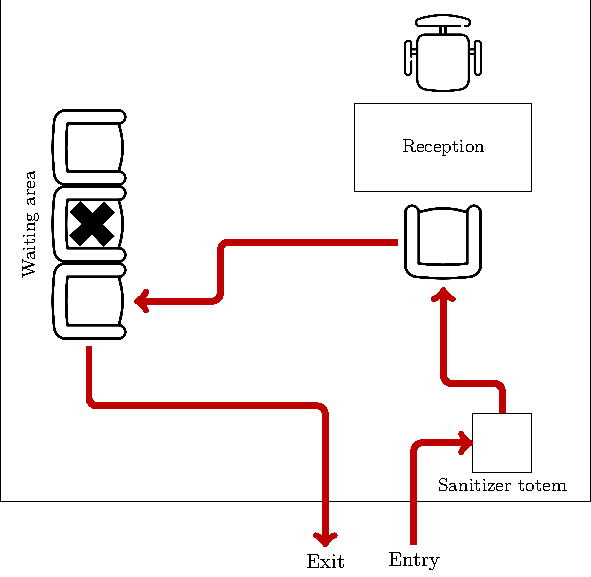
\includegraphics[width = \linewidth]{Metodologia/caminho.pdf}
            \caption{Scheduled task of the experiment and their order.}
            \label{fig:task_diagram}
        \end{figure}
        
        These tasks should engage the user and make it navigate through the room. The purpose is to verify if he/she can draw a mental map of the scene and use the available information about obstacles to avoid them when needed. These sources of distraction were added in order to increase the immersion and to be a distraction as well. Otherwise, the virtual scene would not replicate the reality of a reception scenario.

        Figure \ref{fig:ve_re} shows the virtual environment created in Unity3D and the corresponding real environment assembled at the CCM entrance hall. 
    
        \begin{figure}[!htb]
            \centering
            \begin{subfigure}[b]{0.49\textwidth}
                \centering
                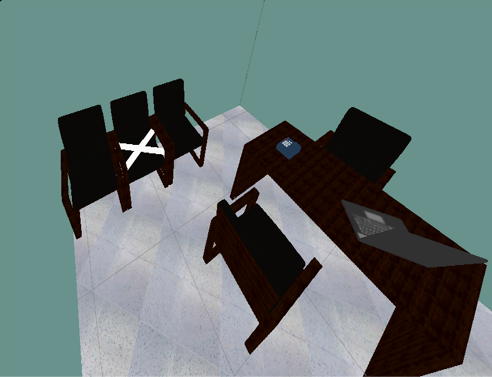
\includegraphics[width=\textwidth]{Metodologia/VE.png}
                \caption{Virtual environment screenshot}
                \label{fig:ve_photo}
            \end{subfigure}
            \hfill
            \begin{subfigure}[b]{0.49\textwidth}
                \centering
                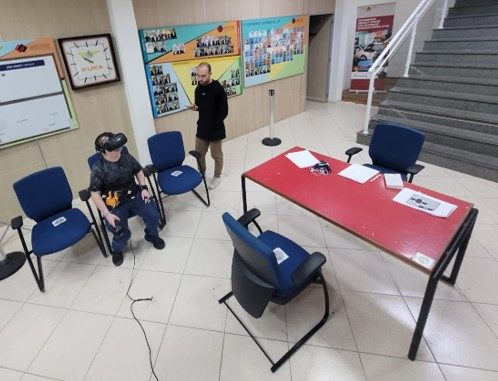
\includegraphics[width=\textwidth]{Metodologia/RE.jpg}
                \caption{Real environment photo}
                \label{fig:re_photo}
            \end{subfigure}
               \caption{Environment comparisson}
               \label{fig:ve_re}
        \end{figure}

    \subsection*{\textit{Step 3.2 Proposal of assessment techniques and tools}}

        As previously defined, the assessment should evaluate performance, workload and situation awareness. Following, we detail the selected techniques and tools for each case.

        \begin{enumerate} [label = \Alph*)]
            \item Performance;
        \end{enumerate}
            
        In the hospital reception scenario, the proposed measurement related to BVI performance is the number of times the BVI user hits the furniture in the virtual environment during the tasks' execution.

        \begin{enumerate} [label = \Alph*)]
            \setcounter{enumi}{1}
            \item Workload;
        \end{enumerate}

        Following the recommendations from the review of literature, the workload is estimated using two approaches:
        \begin{itemize}
            \item Physiological measures obtained from an ECG (Electrocardiogram) sensor and a GSR (Galvanic Skin Response) sensor;
            \item NASA-TLX (National Aeronautics and Space Administration Task Load Index) subjective questionnaire (Appendix \ref{apsec:nasa_tlx}).           
        \end{itemize}

        \begin{enumerate} [label = \Alph*)]
            \setcounter{enumi}{2}
            \item Situation awareness;
        \end{enumerate}

        A modified SAGAT (Situation Awareness Global Assessment Technique) questionnaire is used to evaluate the BVI situation awareness. This questionnaire was based on the proposed idea of \cite{endsley1988design} and is presented in Appendix \ref{apsec:sagat}. The actor acting as the receptionist questioned when the user sat at the reception desk.

        As the original idea, the proposed version is based on 3 levels of situation awareness:

        \begin{enumerate}[leftmargin = 6em, label = Level \arabic* -- ]
            \item Perception
            
            It aims to evaluate if the user can perceive the environment surrounding him/her. It is not expected that the user details about all the objects in the environment, only about some key objects. Example: ”Is there an object around you?”

            \item Comprehension
    
            After the user answer about an detected object, he/she is asked to point to where the object is located. The same question is made when the user moves from the reception desk to the waiting chairs. During this movement, the user needed to find out where are the waiting chairs, and that could make them lose their sense of direction.
    
            \item Projection
            
            This level is measured after every question that asks the location of an object. He/she is then required to answer how far he/she supposes that this object is
            
        \end{enumerate}      

        The questions written for this questionnaire was made with the support of a blind consultant. He was explained about the concept of situation awareness and then suggested questions. The result analysis was based on the number of corrected answers. This adpated SAGAT is on Appendix \ref{apsec:sagat}.

        \begin{enumerate} [label = \Alph*)]
            \setcounter{enumi}{3}
            \item Devices evaluation;
        \end{enumerate}

        Finally, a questionnaire is proposed for evaluating the guidance devices. This questionnaire was also guided by the same blind consultant from the Adapted SAGAT questionnaire. The consultant was asked to make questions about each device that he considered necessary for an assistive device to have and he focused on the comfort, the sense of safety, the sense of confusion and on the precision that the manipulation of the device caused. This questionnaire is on Appendix \ref{apsec:guidace_evaluation}.
        
    \subsection*{\textit{Step 3.3 Development of guidance devices}}

        As previously stated, four guidance methods were proposed to be evaluated in this work.
        
        \begin{enumerate} [label = \Alph*)]
            \item Audio guidance;
            
            The first method is audio guidance. Basically, in the course of the experiment, the participant could give two different voice commands:

            \begin{itemize} [label = --]
                \item “What is around me?”;
            \end{itemize}

            The answer to this command was a quick description of the closest furniture around the user.

            \begin{itemize} [label = --]
                \item “Where is (something)?”.
            \end{itemize}

            The answer to this command was the direction and distance of something asked by the user.

        \end{enumerate}

        Although an automatic audio guidance system that recognizes the two voice commands and answer them could be easily developed, for the proof of concept of the audio guidance system, this was done with the interference of a member of the design team.

        \begin{enumerate} [label = \Alph*)]
            \setcounter{enumi}{1}
            \item Vibration guidance with command – virtual cane;
        \end{enumerate}

        The vibration guidance with command was implemented in a device named "virtual cane", as it was inspired on the long cane. When using a white cane, the user points it to check nearby obstacles in a specific direction. The virtual cane has a similar way of functioning, but instead of connecting the user to the nearby object through the cane, it vibrates when it detects an obstacle in the direction the user pointed it. A virtual reality hand-control was used to implement it. 

        The virtual cane algorithm runs in the virtual environment. When requested by the user, it identifies the nearest object in the direction pointed by the user and calculates its distance. If the nearest object is within a specific range, it then calculates the vibration intensity based on the distance between the object and the user, and sends the corresponding command to the hand-control device.

        \begin{enumerate} [label = \Alph*)]
            \setcounter{enumi}{2}
            \item Vibration guidance without command – haptic belt
        \end{enumerate}

        A haptic belt was developed as a device that uses vibration guidance without command. The belt has appended 8 vibration units that vibrate accordingly to the direction and distance of the closest object around the user. 

        The main differences between the virtual cane and the haptic belt is that the haptic belt checks 360° around the user. When objects are within a certain limit, it vibrates indicating to the user the direction of the closest object. 

        The project of the haptic belt was inspired by a haptic compass \cite{kylecorry31_instructables_2020}. However, instead of having the input being defined by a magnetometer, it uses the information available in the Unity3D environment.

        The haptic belt was developed using an Arduino Mega 2560 and the following materials: an ESP32 DevKit v1, a printed circuit board (PCB), a leather belt, 8 coin vibrators 1027, and a 3D printed case (Figure \ref{fig:case_cinto}). The PCB was designed in the EasyEDA web platform (Figure \ref{fig:pcb_wiring}). 

        \begin{figure}[!htb]
            \centering
            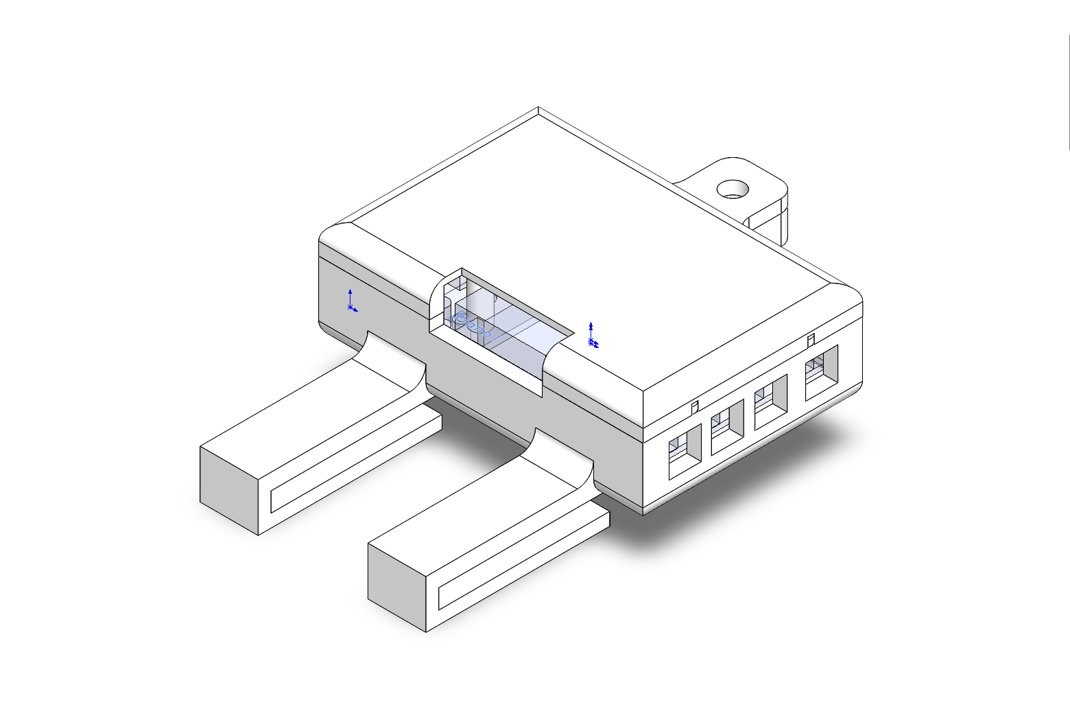
\includegraphics[width = 0.8\linewidth]{Metodologia/Case Cinto.png}
            \caption{CAD model of the designed case}
            \label{fig:case_cinto}
        \end{figure}

        \begin{figure}[htbp]
            \centering
            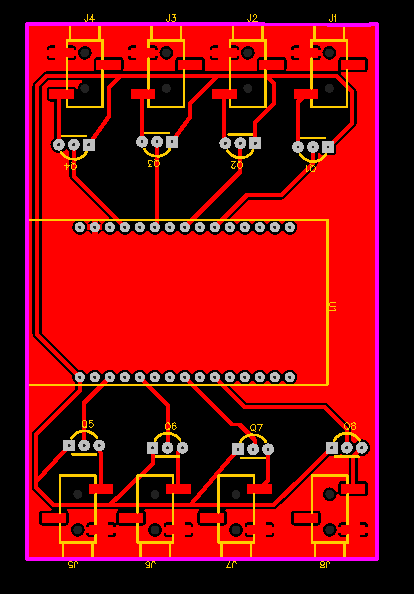
\includegraphics[width=0.45\textwidth, angle = 90, origin = c]{Metodologia/PCB Cinto.pdf}
            \caption{Printed circuit board wiring}
            \label{fig:pcb_wiring}
        \end{figure}

        The haptic belt is illustrated in the Figure \ref{fig:cinto_haptico} and communicates with the Unity3D environment using a Bluetooth connection.

        \begin{figure}[!htb]
            \centering
            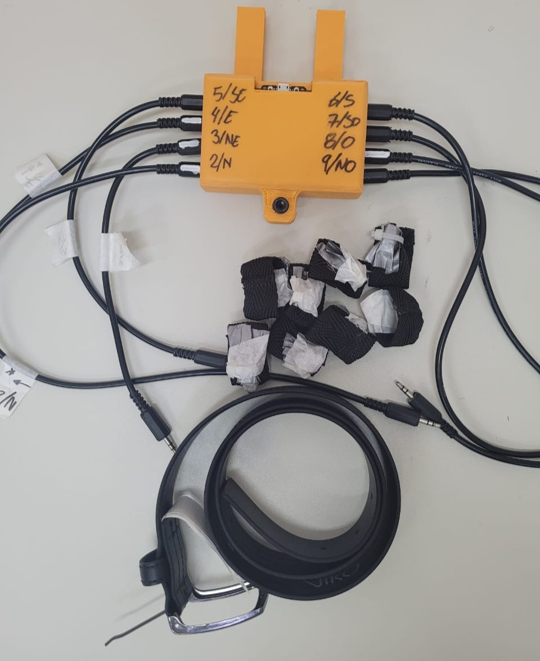
\includegraphics[width = 0.5\linewidth]{Metodologia/Cinto Haptico.png}
            \caption{The haptic belt}
            \label{fig:cinto_haptico}
        \end{figure}

        The haptic belt algorithm is divided into two modules: one implemented in the virtual environment and one implemented in the ESP32 kit. In the virtual environment, it determines the direction of the nearest object to define the vibration motor(s) that must be activated or deactivated and the corresponding intensity. It then sends a message to the ESP32 kit with the corresponding command. The algorithm implemented in the ESP32 kit receives the command from the virtual environment and activates/deactivates the corresponding motors.

        \begin{enumerate} [label = \Alph*)]
            \setcounter{enumi}{3}
            \item Mixture of audio and vibration guidance
        \end{enumerate}

        This option is implemented making the three options available to the user: audio guidance, haptic belt and virtual cane. 


\section{Phase 4 – Preliminary evaluation}
\label{sec:tests_phase}
        
\subsection*{\textit{Step 4.1 Try-out}}

        During the preliminary evaluation phase, the concepts of assistive devices were tested by two BVI users and feedback was provided to improve both the devices and the virtual environment. 

        Regarding the devices, the main feedback provided by the BVI users was about the virtual cane. Initially, the virtual cane algorithm emitted a different sound when the virtual cane was pointed to the floor, walls or ceiling. This sound was found annoying by the BVI users and was removed from the algorithm.

        Regarding the virtual environment, BVI users pointed out the need to add more sources of noise in order to improve the immersion. The suggestions were both for internal and external sounds.
        
        Regarding internal sounds, they point to the lack of people chattering and the noise that came from a TV. Both were included in the virtual environment. In order to simulate people chattering, dialogues between two people, collected from videos or series available on the internet, were added to the virtual environment. The TV noise was collected from famous Brazilian TV programs. Another missing artifact noticed by the team was the queue machine, calling different names at random intervals. 

        Regarding external sounds, the BVI observed that usually they use external sounds to locate the exit of a room. As a suggestion, the following sequence of sound was created and added to the virtual environment to run at random moments:

        \begin{enumerate}
            \item Sound of a door opening;
            \item Noise from an exterior space (like people walking, cars passing by, horns, etc.);
            \item Sound of a door closing.
        \end{enumerate}
        
        The sequence was associated with a sound-emitting point in the virtual environment, running at random moments. 

        Once the preliminary evaluation of the environment was concluded, different versions of the reception were created, modifying the position of the objects, in order to make possible the execution of multiple tests with the same person without the cumulative effect of learning. 

        Another contribution that emerged from the try-out regards detection of the user's collision. A routine was implemented in the virtual environment to detect and register the collisions as a performance metric. The tests with BVI users showed that the routine for automatic collision detection in the virtual world does not work correctly because it does single monitor parts of the human body, such as legs, hands and arms. 

        The only information provided as input is the position and orientation of the head (captured by the HTC VIVE HMD). Based on this information, the virtual platform approximates the volume occupied by the human body to a vertical capsule, as illustrated in Figure \ref{fig:user_straight}. If the user tilts his/her head down, as if facing the ground, the capsule rotates about the HMD point, making the virtual body of the user occupy a different space from user's body, as illustrated in Figure \ref{fig:user_looking_down}. This approximation leads to several errors, both related to detecting collision that did not happened and not detecting collisions that happened.

        \begin{figure}[!htb]
            \centering
            \begin{minipage}{0.45\textwidth}
                \centering
                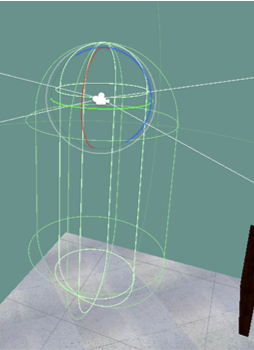
\includegraphics[width = 0.8\linewidth]{Metodologia/envelope1.png}
                \subcaption{The user's capsule while the participant is straight and looking forward.}
                \label{fig:user_straight}
            \end{minipage}
            \begin{minipage}{0.075\textwidth}
                \hfill
            \end{minipage}
            \begin{minipage}{0.45\textwidth}
                \centering
                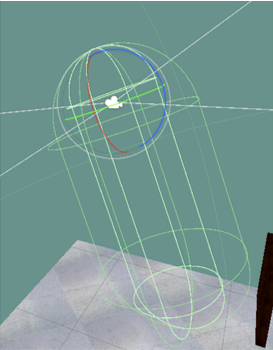
\includegraphics[width = 0.8\linewidth]{Metodologia/envelope2.png}
                \subcaption{The user's capsule while the participant is straight but looking down.}
                \label{fig:user_looking_down}
            \end{minipage}
            \caption{Two different capsule positions based on the user's head position.}
            \label{fig:user_envelope}
        \end{figure}

\section{Phase 5 – Systematic evaluation}
\label{sec:experiment}
        
During the systematic evaluation phase, the evaluation experiment is designed and executed. It consists of inviting BVI volunteers to use the assistive devices to navigate inside the virtual environment and perform the proposed tasks. The assessment techniques are applied during and after the use of each device.

In the case of this work, the proposed experiment consists of asking the participant to use five guidance methods: the four methods presented in Section \ref{sec:idealization_phase} (audio guidance, haptic belt, virtual cane, mixed) and, additionally, the device used daily by the BVI (e.g., white cane). Moreover, each participant should use each guidance method twice (“first visit” and “return visit”), in order to provide some information about how the guidance devices performs in new and known environments.

In order to avoid the learning effect from one method to the other, five versions of the reception scene are developed, changing the position of the objects - one version to be used with each guidance method. The scene order is randomized for each participant.

Moreover, particularly in the case of this work, an additional round of tests is added to the experiment to investigate the differences between the evaluation performed by BVI users and sighted (non-BVI) users. For this purpose, the same experiment is repeated with a set of non-BVI users. The purpose is to investigate whether or not performing the analysis with non-BVI users could lead to different conclusions.

The experiment is organized in the following way:

\begin{itemize}
    \item Briefing:
    \begin{itemize}
        \item The experiment's purpose is explained to the participant, followed by the signature or recording of the free and informed consent form.
        \item An explanation about the physiological sensor is provided and the participant is invited to wear it.
        \item The assistive devices are introduced to the participant.
        \item The participant is invited to wear the VIVE HMD and start the experiment. 
    \end{itemize}
    \item Execution of the experiment - the following sequence is repeated for each guidance method:
    \begin{itemize}
        \item The participant receives a brief introduction about the guidance method and is given some time to familiarize and train with it. During this step, no data is gathered. 
        \item First visit: the participant performs the task and is asked the SAGAT questionnaire during the task.
        \item The participant answers the NASA-TLX for the first visit.
        \item Return visit: the participant performs the task for the second time in the same scene. However, a few things are changed, such as the presence, or not, of a television or random people talking. The participant answers the SAGAT questionnaire again.
        \item The participant answers the NASA-TLX for the return visit.
        \item After both visits, the participant answers the questionnaire about the guidance method.
    \end{itemize}
    \item Conclusion
    \begin{itemize}
        \item The physiological sensors are removed from the participant and the experiment is concluded.
    \end{itemize}
\end{itemize}

As a result of the experiment, the following data are collected:

\begin{itemize}
    \item Answers to the NASA-TLX questionnaire (Appendix \ref{apsec:nasa_tlx});
    \item ECG and GSR signals;
    \item Answers to the SAGAT questionnaire (Appendix \ref{apsec:sagat});
    \item Answers to the guidance method questionnaire (Appendix \ref{apsec:guidace_evaluation}).
\end{itemize}

The data analysis is discussed in the next chapter.

\section{Final Remarks}

This chapter describes the proposed method in this work to evaluate early concepts of assistive devices using virtual reality using the proposed set of assessment techniques. 

The next chapter shows the results obtained from the execution of an experimental campaign.